\documentclass[border=0.2cm,convert]{standalone}
\usepackage{tikz}

% xelatex --shell-escape *.tex

\tikzset{level distance=2em}
\tikzset{level 1/.style = {sibling distance = 3cm}}
\tikzset{level 2/.style = {sibling distance = 2cm}}
\tikzset{every node/.style={draw,circle}}
\tikzset{blank/.style={draw=none}}

\begin{document}

\begin{tabular}{cc}
$1.$ Vorher & $2.$ $33$ gelöscht \\
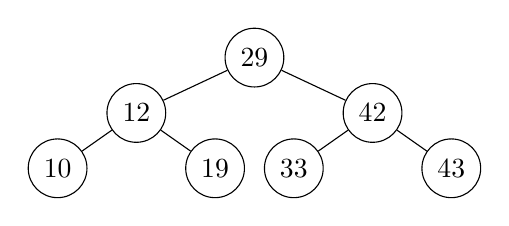
\begin{tikzpicture}
\node{29}
    child {
        node {12}
        child {node{10}}
        child {node{19}}
    }
    child {
        node {42}
        child {node{33}}
        child {node{43}}
    };
\end{tikzpicture}
&
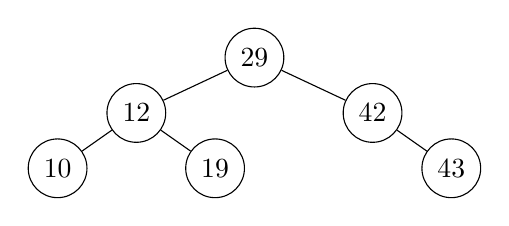
\begin{tikzpicture}
\node{29}
    child {
        node {12}
        child {node{10}}
        child {node{19}}
    }
    child {
        node {42}
        child [transparent] {node{}}
        child {node{43}}
    };
\end{tikzpicture}
\\

$3.$ $42$ gelöscht & $4.$ $29$ gelöscht \\
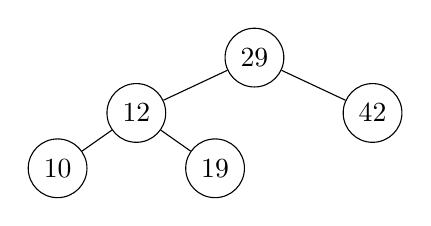
\begin{tikzpicture}
\node{29}
    child {
        node {12}
        child {node{10}}
        child {node{19}}
    }
    child {node {42}}
    ;
\end{tikzpicture}
&
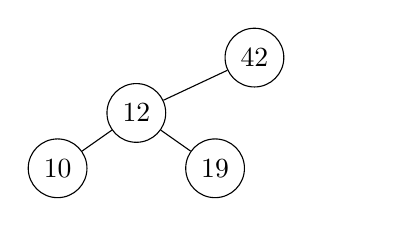
\begin{tikzpicture}
\node{42}
    child {
        node {12}
        child {node{10}}
        child {node{19}}
    }
    child [transparent] {node{}}
    ;
\end{tikzpicture}

\end{tabular}
\end{document}
